\chapter{Implementation}

In this chapter the implementation details will be described.
For this, first the used technologies are explained.
After this, the database schema that was used for storing the meta-features and the evaluations will be described.
Last but not least the used algorithms, optimizers and features will be mentioned.

\section{Technologies}

\begin{itemize}
    \item Python as programming language
    \item scikit-learn \cite{PedregosaFABIANPEDREGOSA2011Scikit-learn:Perrot} as library for implementing the algorithms and the metrics.
    \item Used algorithms KMeans, KMedoids\cite{Kaufman1987ClusteringMedoids} and GMM. 
    Implementations taken from scikit-learn, besides KMedoids which was taken from scikit-learn extra\footnote{https://scikit-learn-extra.readthedocs.io/en/latest/user_guide.html#k-medoids}.
    \item For all algorithms the number of max iterations were set to 10.
    \item KMeans was implemented using the  \textit{k-means++} \cite{Arthur2007K-means++:Seeding} method
    and KMedoids with a similar method, called \textit{k-medoids++}.
    \item The metrics that were used were all that are implemented in scikit-learn, which means 6 external and 3 internal were used.
    \item The Silhouette coefficient \cite{Rousseeuw1987Silhouettes:Analysis} was implemented using only 10\% of the data with random sampling.
    \item The reason is the high runtime which would exceed the possibilities and resources of this work.
    \item For the online phase only the 3 internal metrics were used. 
    \item The optimizers that were used were all that were described in ... \xtodo{reference here background section of optimizers}
    \item The implementation of the Random and the Bayes optimizer was done using the scikit-optimize \cite{Head2018Scikit-optimize} implementation.
    \item Reason for this library: in python, easy to add warmstarting, ask-and-tell interface.
    \item The Hyperband and BOHB optimizers were implemented using the implementation mentioned in \cite{Falkner2018BOHB:Scale}, which contains an implementation for both Hyperband and BOHB.
    \item The architecture was kept quite flexible so that running each optimizer which each metric on each implemented algorithm is possible.
    \item Goal is to compare the different optimizers and metrics per optimizer.
    \item Relational database was used because the relationship between the metafeatures, dataset and the results of the optimizers need to be stored.
    \item Also the schema should not change.
    \item PostgreSQL\footnote{https://www.postgresql.org/} used as database.
    \item The meta-feature extraction was done using the pymfe\footnote{https://pypi.org/project/pymfe/} \cite{Rivolli2018TowardsMeta-learning} package.
    \item For this all meta-features were used that do not need class labels.
\end{itemize}

\section{Database Schema}
\begin{itemize}
    \item For accessing the PostgreSQL database instance, the python package SQLAlchemy \cite{sqlalchemy} was used.
    \item More specific, the Object-relational mapper was used.
    \item Schema of the database is shown in \cref{fig:dbschema}.
    Describe in more detail.
    \begin{figure}
        \centering
        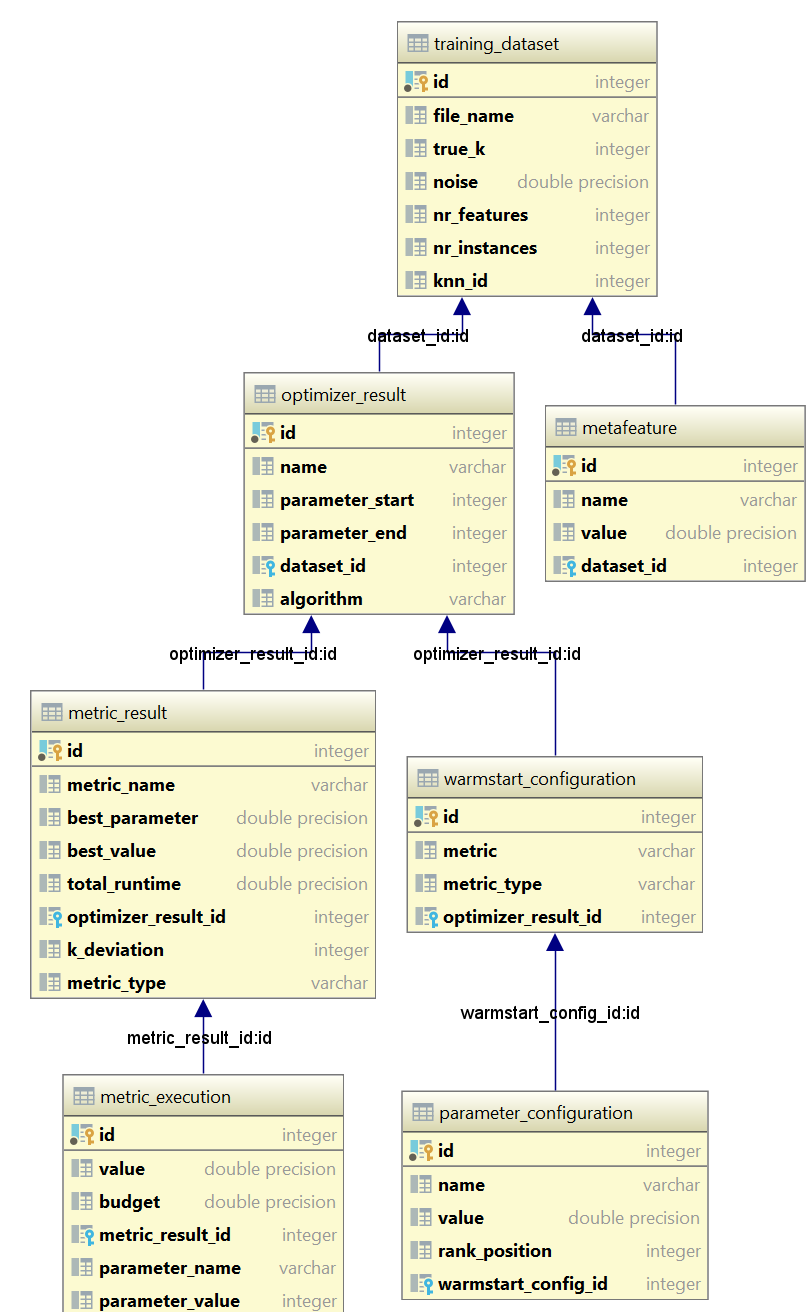
\includegraphics[width=0.7\textwidth]{graphics/database_schema.png}
        \caption{Overview of the database schema that was used to store the meta-features as well as the results of the optimizers.}
        \label{fig:dbschema}
    \end{figure}
    
    \xtodo{Show schema for algo selection as well and explain difference? But actually not that much changed...}
\end{itemize}

\section{Generation of Training and Test Datasets}

In this section the datasets that were used for the evaluation will be described.
\begin{itemize}
    \item For Offline phase of the concept, training data is needed.
    \item Introduce notation
    \item 
\end{itemize}


